\documentclass[12pt,a4paper]{article}

% --- Настройка языка и шрифтов для LuaLaTeX ---
\usepackage{fontspec}
\defaultfontfeatures{Ligatures=TeX,Scale=MatchLowercase}

\setmainfont{Alice-Regular}[
    Path=font/,
    Extension=.ttf,
    BoldFont = Alice-Regular,
    ItalicFont = Alice-Regular,
    BoldItalicFont = Alice-Regular,
    BoldFeatures = {FakeBold=1.6},
    ItalicFeatures = {FakeSlant=0.2},
    BoldItalicFeatures = {FakeBold=1.6,FakeSlant=0.2}
]

\newfontfamily\cyrillicfont{Alice-Regular}[
    Path=font/,
    Extension=.ttf,
    BoldFont = Alice-Regular,
    ItalicFont = Alice-Regular,
    BoldItalicFont = Alice-Regular,
    BoldFeatures = {FakeBold=1.6},
    ItalicFeatures = {FakeSlant=0.2},
    BoldItalicFeatures = {FakeBold=1.6,FakeSlant=0.2}
]

\usepackage{polyglossia}
\setmainlanguage{russian}
\setsansfont{TeX Gyre Heros}
\setmonofont{TeX Gyre Cursor}

\usepackage{graphicx}        					          % Графика
\usepackage[protrusion=false]{microtype}       	% Микротипографика
\usepackage{amsmath, amsfonts, amssymb, amsthm}	% Математика
\usepackage{braket} 							              % Braket нотация для квантовой механики
\usepackage{unicode-math} 						          % Современный пакет для математики в LuaLaTeX
\usepackage{longtable}       					          % Таблицы с разрывом страниц
\usepackage{tikz}           					          % Рисование
\usepackage[europeanresistors]{circuitikz}		  % Рисование электрических схем в европейском стиле
\usepackage{listings}							              % Для отображения кода
\usepackage{tabularx}       					          % Для таблиц во всю ширину
\usepackage{array}		  						            % Для расширенных возможностей таблиц
\usepackage{float}          					          % Для точного позиционирования фигур
\usepackage{pgfplots}                           % Для построения графиков
\usepackage{caption}                            % Для настройки подписей к рисункам и таблицам
\usepackage{xfp}                                % Для вычислений в LaTeX
\pgfplotsset{compat=1.18}
\usepackage[a4paper,left=20mm,right=20mm,top=20mm,bottom=20mm]{geometry}

\usetikzlibrary{arrows.meta}

% --- Колонтитулы ---
\usepackage{fancyhdr}
\pagestyle{fancy}
\fancyhf{}

\renewcommand{\headrulewidth}{0.4pt}
\renewcommand{\footrulewidth}{0.4pt}
\renewcommand\lstlistingname{Исходный код}

\lstdefinestyle{main}{
	backgroundcolor=\color{gray!8},   
	commentstyle=\color{green!50!black},
	keywordstyle=\color{blue!80!black},
	numberstyle=\small\color{darkgray},
	stringstyle=\rmfamily\color{orange!90!black},
	basicstyle=\ttfamily\small,
	breakatwhitespace=false,         
	breaklines=true,                   
	keepspaces=true,                 
	numbers=left,                    
	numbersep=8pt,                  
	showspaces=false,                
	showstringspaces=false,
	showtabs=false,                  
	tabsize=4
}	

\lstset{style=main}

\newcolumntype{C}{>{\centering\arraybackslash}X}
\renewcommand{\arraystretch}{1.25}

% =========================================================
%         СЛУЖЕБНЫЕ КОМАНДЫ ДЛЯ ВЫЧИСЛЕНИЙ
% =========================================================
\newcommand{\CalcZero} [1]{\fpeval{round((#1),0)}}
\newcommand{\CalcOne}  [1]{\fpeval{round((#1),1)}}
\newcommand{\CalcTwo}  [1]{\fpeval{round((#1),2)}}
\newcommand{\CalcThree}[1]{\fpeval{round((#1),3)}}
\newcommand{\CalcFour} [1]{\fpeval{round((#1),4)}}
\newcommand{\CalcFive} [1]{\fpeval{round((#1),5)}}

% ---------------------------------------------------------
% ОБЩИЕ ДАННЫЕ
% ---------------------------------------------------------
\def\LabNumber {1}					% Номер лабораторной работы
\def\Discipline{Квантовая Механика} % 
\def\LabTitle  {Коллоквиум}

\title{
	МИНОБРНАУКИ РОССИИ

	федеральное государственное автономное образовательное учреждение

	высшего образования

	«Национальный исследовательский университет
	«Московский институт электронной техники»
	\vspace{2em}
}
\author{
}
\date{}

\begin{document}

\maketitle
\thispagestyle{fancy}

\begin{center}
\Large Отчёт по Лабораторной работе $\LabNumber$\\
по дисциплине «\Discipline»\\
«\LabTitle»
\end{center}

\vspace{12em}

\cfoot{Москва 2026}

\pagebreak

\fancyhead[L]{\LabTitle} 
\fancyhead[R]{\Discipline} 
\fancyfoot[C]{\thepage} 

\section{Экспериментальные основы квантовой механики}

% Классическая механика Ньютона не могла описать процессы, происходящие в микросистемах.
% Габариты системы удобно определять порядком действия в ней, если действие $S \gg h$, то
% это макросистема, если $S \sim h$, то это микросистема.

Габариты системы стандартной и квантовой модели

\begin{equation*}
	S \gg h \qquad S \sim h
\end{equation*}

Формула Рэлея-Джинса

\begin{equation*}
	I(\omega) = \frac{\omega^2}{4\pi^2c^2}kT
\end{equation*}

Формула Планка

\begin{equation*}
	I(\omega) = \frac{\omega^2}{4\pi^2c^2}\frac{h\omega}{e^\frac{h\omega}{kT} - 1}	
\end{equation*}

\begin{center}
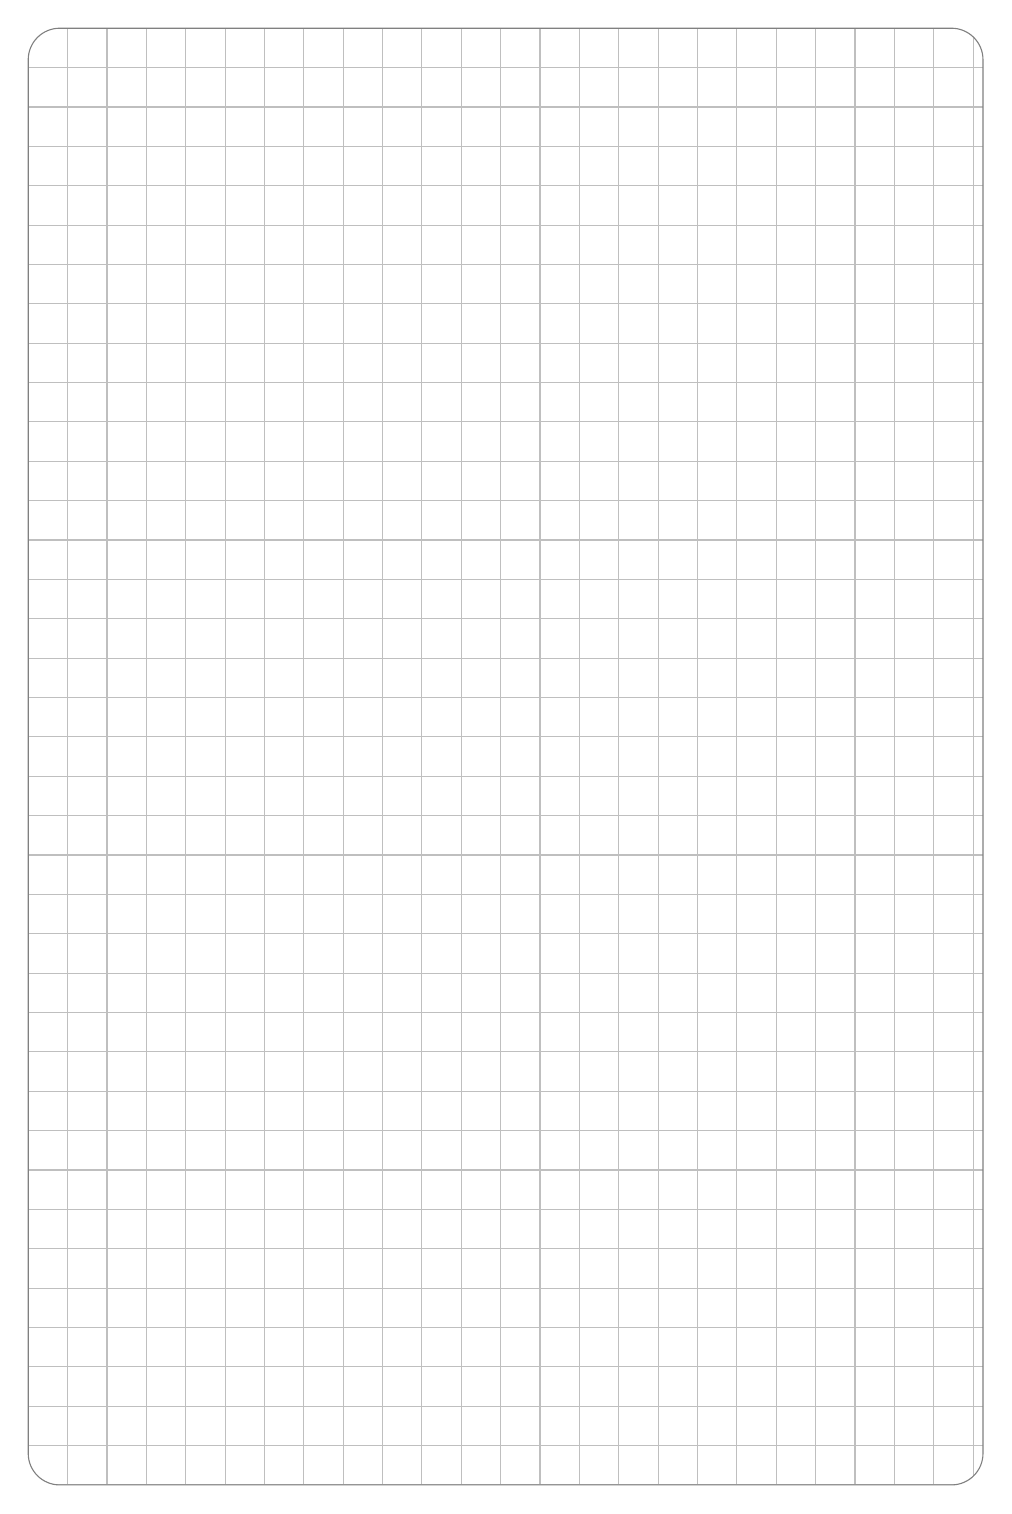
\begin{tikzpicture}
    % параметры
    \def\W{\textwidth}     % ширина прямоугольника
    \def\H{37 * 5mm} % высота прямоугольника
    \def\R{4mm}     	   % радиус скругления
    \def\S{5mm}     	   % шаг сетки

    % обрезаем всё по прямоугольнику со скруглёнными углами
    \begin{scope}
        \clip[rounded corners=\R] (0,0) rectangle (\W,\H);

        % тетрадная сетка
        \draw[step=\S, thin, gray!50] (0,0) grid (\W,\H);
    \end{scope}

    % внешний контур
    \draw[rounded corners=\R, gray] (0,0) rectangle (\W,\H);
\end{tikzpicture}
\end{center}

\section[short]{Принцип неопределённости}

Принцип неопределённости Гейзенберга

\begin{equation*}
	\Delta A \Delta B \ge \frac{C}{2}
\end{equation*}


\begin{center}
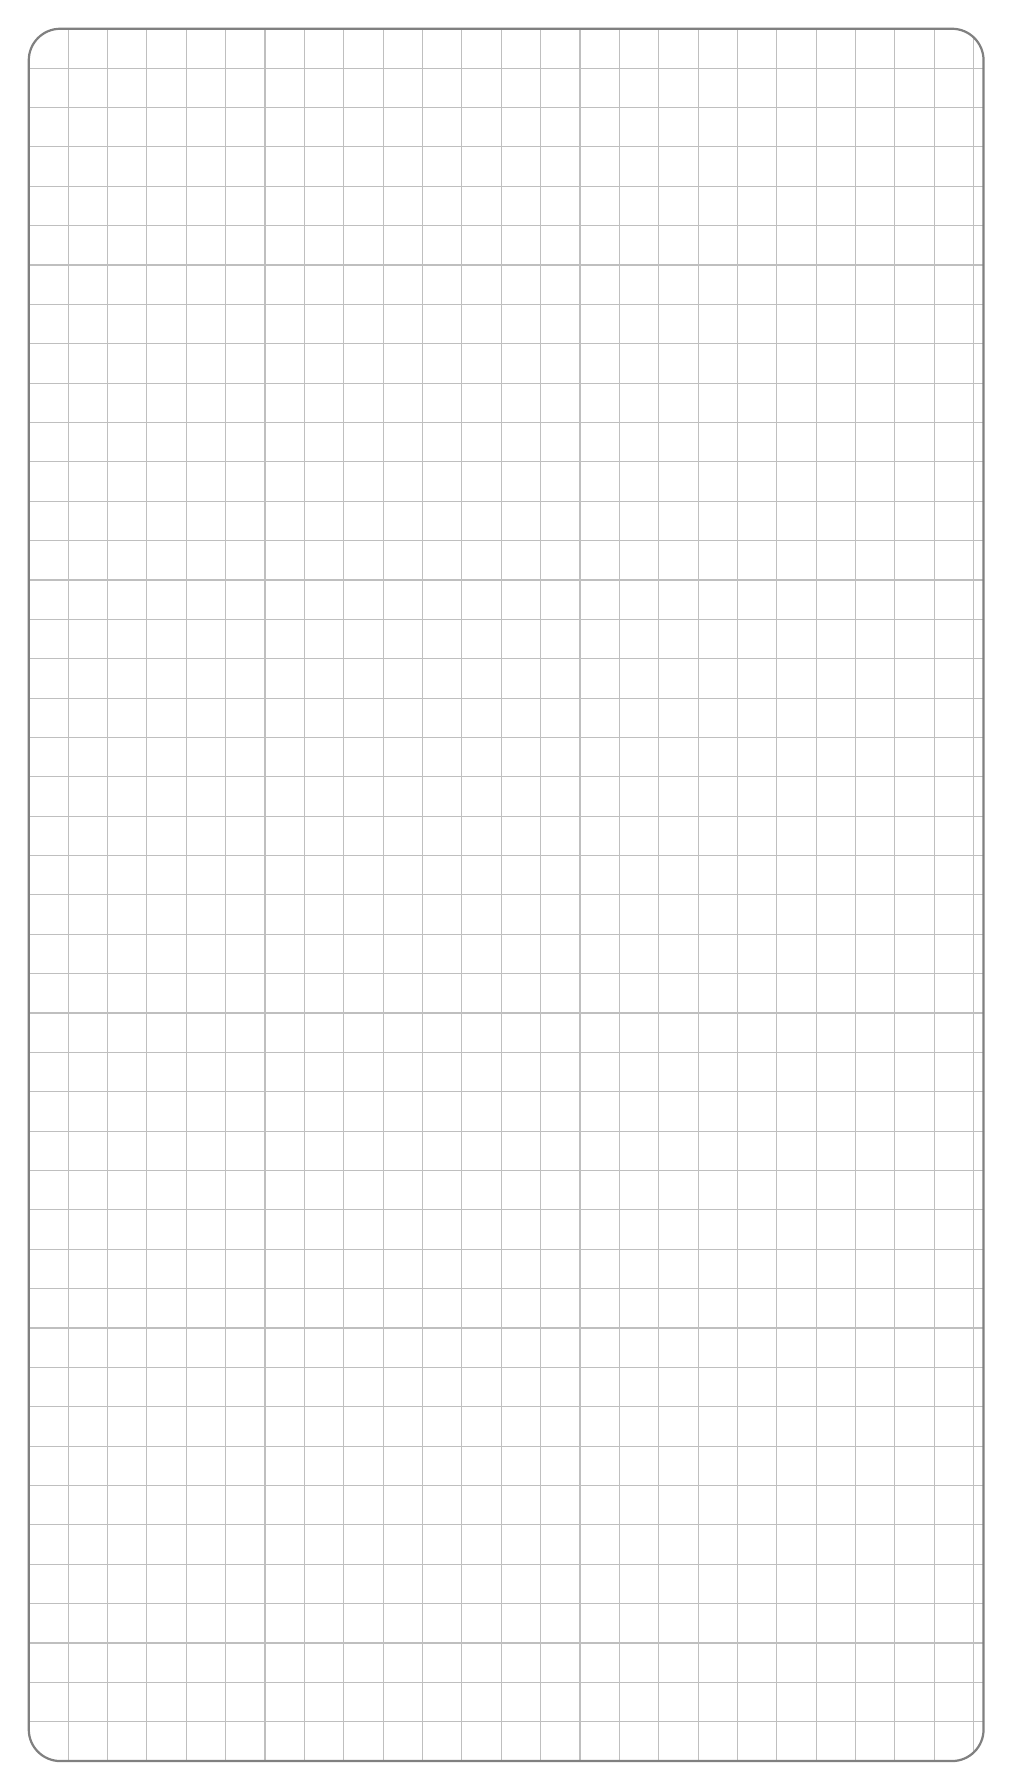
\begin{tikzpicture}
    % параметры
    \def\W{\textwidth}     % ширина прямоугольника
    \def\H{44 * 5mm} % высота прямоугольника
    \def\R{4mm}     	   % радиус скругления
    \def\S{5mm}     	   % шаг сетки

    % обрезаем всё по прямоугольнику со скруглёнными углами
    \begin{scope}
        \clip[rounded corners=\R] (0,0) rectangle (\W,\H);

        % тетрадная сетка
        \draw[step=\S, thin, gray!50] (0,0) grid (\W,\H);
    \end{scope}

    % внешний контур
    \draw[rounded corners=\R, line width=0.8pt, gray] (0,0) rectangle (\W,\H);
\end{tikzpicture}
\end{center}

\section[short]{Полный набор динамических переменных}

\section[short]{Волновая функция и её свойства}

\section[short]{Принцип суперпозиции состояний}

\section[short]{Запутанные квантовые состояния}

\section[short]{Среднее значение измеряемой величины и вероятность результатов её измерения}

\section[short]{Операторы коордитнаты, импульса, момента импульса, энергии}

\section[short]{Решение задачи на собственные функции и собственные значения для 
оператора импульса}

\section[short]{Решение задачи на собственные функции и собственные значения 
для оператора проекции момента импульса на выделенную ось}

\section[short]{Коммутаторы и одновременная измеримость физических величин. 
Вычисление коммутаторов, содержищих операторы коордитнаты импульса, момента импульса}

\section[short]{Волновое уравнение}

\section[short]{Оператор Галмильтона различных систем: свободный электрон, электрон в 
кулоновском потенциале, электрон в постоянном электрическом поле, молекула водорода}

\section[short]{Решение волнового уравнения в случае свободной материальной точки}

\section[short]{Вычисление временной части волновой функции стационрного состояния}

\section[short]{Вычислить волновую функцию и энергитический спектр электрона в бесконечно 
глубокой потенциальной яме}

\section[short]{Квантовый гармонический осциллятор: гамильтониан, волновая функция и 
энергитический спектр}

\section[short]{Электрон в магнитном поле: циклотронная частота, гамильтониан, 
вектор-потенциал магнитного поля, уровни Ландау}

\section[short]{Уравнение Шрёдингера для электрона в постоянном электрическом поле. 
Решение в импульсном представлении.}

\section[short]{Плотность потока вероятности. Вычисление плотности потока вероятности
в случае свободной материальной точки}

\section[short]{Коэффициэнт прохождения потока электронов. Туннельный эффект. 
Вычисление прозрачности барьера в виде дельта-функции.}

\section[short]{Спин. Оператор спина. Опыт Штерна-Герлаха. Одновременная 
измеримость различных проекций спина.}

\section[short]{Спинновая переменная волновой функции. Симметричные и 
антисимметричные состояния}

\section[short]{Матрицы Паули}

\section[short]{Фермионы и бозоны (привести примеры частиц). Тождественность 
квантовых частиц. Запрет Паули. Бозе конденсация.}

\section[short]{Волновые функции систем невзаимодействующих бозонов и 
фермионов, детерминант Слеттера}

\section[short]{Стационнарная теория возмущений, первое приближение, 
условие применимости}

\end{document}